%-------- Important LaTeX keyboard shortcuts-------
% Ctrl + Alt + B  Build/compile LaTeX PDF
% Ctrl + Alt + V  Open LaTeX PDF preview

\documentclass[11pt,a4paper]{article}

\usepackage[margin=2.4cm]{geometry}
\usepackage{amsmath,amssymb,amsthm}
\usepackage{enumitem}
\usepackage{booktabs}
\usepackage{array}
\usepackage{tikz}
\usepackage{hyperref}

\hypersetup{colorlinks=true, linkcolor=black, urlcolor=blue}

\newcommand{\T}{\ensuremath{\mathrm{T}}}
\newcommand{\F}{\ensuremath{\mathrm{F}}}
\newcommand{\iimplies}{\rightarrow}
\newcommand{\iiff}{\leftrightarrow}

\setlist[enumerate]{itemsep=2pt, topsep=4pt}

\title{CITS2211 Discrete Structures \\ Assignment One}
\author{Atulya}
\date{Semester 2, 2026}

\begin{document}
\maketitle

\section*{Question 1}

\textbf{Claim.} $\neg P \vee \neg Q \iiff \neg P \vee (\neg Q \wedge P)$ is a tautology.

\medskip
\noindent Write $L = \neg P \vee \neg Q$ and $R = \neg P \vee (\neg Q \wedge P)$.

\begin{center}
\begin{tabular}{cc|cc|c|c|c|c}
\toprule
$P$ & $Q$ & $\neg P$ & $\neg Q$ & $L = \neg P \vee \neg Q$ & $\neg Q \wedge P$ & $R = \neg P \vee (\neg Q \wedge P)$ & $L \iiff R$ \\
\midrule
\T & \T & \F & \F & \F & \F & \F & \T \\
\T & \F & \F & \T & \T & \T & \T & \T \\
\F & \T & \T & \F & \T & \F & \T & \T \\
\F & \F & \T & \T & \T & \F & \T & \T \\
\bottomrule
\end{tabular}
\end{center}

The final column is $\T$ in every row, so the proposition is true under every truth assignment. Hence it is a tautology. $\blacksquare$

\section*{Question 2}

\textbf{Claim.} $(P \iimplies Q) \vee (\neg Q \wedge P)$ is a tautology.

\begin{align*}
(P \iimplies Q) \vee (\neg Q \wedge P)
&\equiv (\neg P \vee Q) \vee (\neg Q \wedge P) && \text{Implication law} \\
&\equiv \bigl((\neg P \vee Q) \vee \neg Q\bigr) \wedge \bigl((\neg P \vee Q) \vee P\bigr) && \text{Distributive law} \\
&\equiv \bigl(\neg P \vee (Q \vee \neg Q)\bigr) \wedge \bigl((Q \vee \neg P) \vee P\bigr) && \text{Associative and Commutative laws} \\
&\equiv \bigl(\neg P \vee (Q \vee \neg Q)\bigr) \wedge \bigl(Q \vee (\neg P \vee P)\bigr) && \text{Associative law} \\
&\equiv (\neg P \vee \T) \wedge (Q \vee \T) && \text{Negation (complement) law} \\
&\equiv \T \wedge \T && \text{Domination law} \\
&\equiv \T && \text{Idempotent (or Identity) law}
\end{align*}

Since the expression reduces to $\T$, it is a tautology. $\blacksquare$

\section*{Question 3}

An inference rule is \emph{sound} if every truth assignment that makes all premises true also makes the conclusion true.

\begin{enumerate}[label=\alph*)]
\item $\dfrac{P}{Q}$ --- \textbf{Unsound.} Counterexample: $P = \T$, $Q = \F$. The premise is true, the conclusion is false.

\item $\dfrac{P \quad Q}{P \vee Q}$ --- \textbf{Sound.} If both premises are true then in particular $P = \T$, and a disjunction is true whenever at least one disjunct is true, so $P \vee Q = \T$. (This is $\vee$-introduction with a redundant second premise.)

\item $\dfrac{P}{P \iiff Q}$ --- \textbf{Unsound.} Counterexample: $P = \T$, $Q = \F$. Premise true, but $\T \iiff \F = \F$.

\item $\dfrac{P \quad Q}{P \iiff Q}$ --- \textbf{Sound.} If both premises hold then $P = Q = \T$, and $\T \iiff \T = \T$. More generally the biconditional is true whenever both sides have the same truth value.

\item $\dfrac{\neg P \quad P \vee P}{Q}$ --- \textbf{Sound (vacuously).} By idempotence $P \vee P \equiv P$, so the premises are $\neg P$ and $P$. No truth assignment makes both true, so there is no assignment that makes all premises true and the conclusion false. The rule is therefore truth-preserving. This is the principle of explosion: contradictory premises entail anything.
\end{enumerate}

\section*{Question 4}

\textbf{Premises.} (1) $\neg\neg P \vee Q$ \quad (2) $P \iiff R$ \quad (3) $H \iimplies \neg Q$. \quad \textbf{Goal.} $H \iimplies P$.

\begin{center}
\begin{tabular}{r l l}
\toprule
\# & Formula & Justification \\
\midrule
1 & $\neg\neg P \vee Q$ & Premise \\
2 & $P \iiff R$ & Premise \\
3 & $H \iimplies \neg Q$ & Premise \\
4 & $H$ & Assumption (for conditional proof) \\
5 & $\neg Q$ & Modus ponens, 3 and 4 \\
6 & $\neg\neg P$ & Disjunctive syllogism, 1 and 5 \\
7 & $P$ & Double negation elimination, 6 \\
8 & $H \iimplies P$ & $\iimplies$-introduction (conditional proof), discharging 4 \\
\bottomrule
\end{tabular}
\end{center}

\medskip
\noindent\textbf{Observation.} Premise (2), $P \iiff R$, is never used. It is redundant: the proposition letter $R$ does not occur in the conclusion, and no step of the derivation depends on it, so the conclusion follows from premises (1) and (3) alone. The double negation in premise (1) is also redundant, since $\neg\neg P \vee Q \equiv P \vee Q$, which would remove the need for line 7.

\section*{Question 5}

Domain: $\mathbb{N}$. $P(n)$ means ``$n$ is prime''.

\begin{enumerate}[label=(\alph*)]
\item $\exists n.\, P(n)$ \\
``There is at least one prime number.''

\item $\forall n.\, P(n) \iimplies \neg P(2n)$ \\
``For every prime number $n$, twice $n$ is not prime.'' (Equivalently: no prime has a prime double. This is true, since $2n$ is even and greater than $2$.)

\item $\forall n.\, \exists x.\, x > n \wedge P(x) \wedge P(x+2)$ \\
``However far along the number line you go, there is always a larger pair of primes differing by two.'' That is, there are infinitely many twin primes. (This is the Twin Prime Conjecture, still open.)

\item There exists a prime number greater than 30:
\[ \exists n.\, \bigl(n > 30 \wedge P(n)\bigr) \]

\item Every prime number greater than 2 is odd:
\[ \forall n.\, \bigl(P(n) \wedge n > 2\bigr) \iimplies \neg \exists k.\, (n = 2k) \]
Equivalently, stating oddness positively:
\[ \forall n.\, \bigl(P(n) \wedge n > 2\bigr) \iimplies \exists k.\, (n = 2k + 1) \]
\end{enumerate}

\section*{Question 6}

\textbf{Claim.} For all $a \in \mathbb{Z}$, if $a^3$ is even then $a - 1$ is odd.

\medskip
\noindent\textbf{Contrapositive.} For all $a \in \mathbb{Z}$, if $a - 1$ is \emph{not} odd (i.e.\ $a-1$ is even) then $a^3$ is \emph{not} even (i.e.\ $a^3$ is odd).

\medskip
\noindent\textbf{Proof.} Let $a \in \mathbb{Z}$ and suppose $a - 1$ is even.

\begin{enumerate}
\item By the definition of even, there exists $k \in \mathbb{Z}$ with $a - 1 = 2k$.
\item Rearranging, $a = 2k + 1$, so $a$ is odd.
\item Cubing:
\[
a^3 = (2k+1)^3 = 8k^3 + 12k^2 + 6k + 1 = 2\bigl(4k^3 + 6k^2 + 3k\bigr) + 1 .
\]
\item Since $k \in \mathbb{Z}$ and $\mathbb{Z}$ is closed under multiplication and addition, $m := 4k^3 + 6k^2 + 3k \in \mathbb{Z}$.
\item Therefore $a^3 = 2m + 1$ with $m \in \mathbb{Z}$, which is the definition of $a^3$ being odd. Hence $a^3$ is not even.
\end{enumerate}

The contrapositive holds for arbitrary $a \in \mathbb{Z}$, and a conditional is logically equivalent to its contrapositive, so the original statement holds for all $a \in \mathbb{Z}$. $\blacksquare$

\section*{Question 7}

\textbf{Claim.} For all $n \in \mathbb{N}$ with $n \geq 1$,
\[
\sum_{i=1}^{n} i^3 = \frac{n^2 (n+1)^2}{4}.
\]

\noindent Let $S(n)$ denote this statement.

\medskip
\noindent\textbf{Base case ($n = 1$).}
\[
\text{LHS} = \sum_{i=1}^{1} i^3 = 1^3 = 1, \qquad
\text{RHS} = \frac{1^2 \cdot 2^2}{4} = \frac{4}{4} = 1 .
\]
So $S(1)$ holds.

\medskip
\noindent\textbf{Inductive step.} Let $k \geq 1$ and assume $S(k)$, i.e.\ $\displaystyle\sum_{i=1}^{k} i^3 = \frac{k^2(k+1)^2}{4}$. Then
\begin{align*}
\sum_{i=1}^{k+1} i^3
&= \left( \sum_{i=1}^{k} i^3 \right) + (k+1)^3 && \text{splitting off the last term} \\
&= \frac{k^2(k+1)^2}{4} + (k+1)^3 && \text{inductive hypothesis} \\
&= \frac{k^2(k+1)^2 + 4(k+1)^3}{4} \\
&= \frac{(k+1)^2 \bigl[\, k^2 + 4(k+1) \,\bigr]}{4} && \text{factor out } (k+1)^2 \\
&= \frac{(k+1)^2 \bigl(k^2 + 4k + 4\bigr)}{4} \\
&= \frac{(k+1)^2 (k+2)^2}{4} .
\end{align*}
This is exactly the claimed formula with $n = k+1$, so $S(k) \Rightarrow S(k+1)$.

\medskip
By the principle of mathematical induction, $S(n)$ holds for all $n \geq 1$. $\blacksquare$

\section*{Question 8}

\textbf{Claim.} A square can be dissected into $n$ smaller squares (with disjoint interiors, covering the whole square) for every $n \in \mathbb{N} \setminus X$, where
\[
\boxed{X = \{2, 3, 5\}}
\]

\subsection*{Part A: the impossible cases}

\textbf{Key lemma.} If a square is dissected into $n \geq 2$ squares, then each of the four corners of the large square is a corner of a distinct small square, so $n \geq 4$.

\medskip
\noindent\emph{Proof.} Each corner point of the large square lies in some small square, and must be a corner of it. A small square containing two corners of the large square would have to span an entire side, hence have the same side length as the large square, hence be the large square itself, contradicting $n \geq 2$. So the four corners lie in four different small squares, giving $n \geq 4$. $\square$

\medskip
This immediately rules out $n = 2$ and $n = 3$. ($n = 0$ is excluded trivially; $n = 1$ is the square itself.)

\medskip
\noindent\textbf{The case $n = 5$ is impossible.} Suppose the large square has side $s$ and is dissected into $5$ squares. By the lemma, four of them are corner squares. Let their side lengths be $a$ (bottom-left), $b$ (bottom-right), $c$ (top-left), $d$ (top-right). The fifth square is the only one left over.

\begin{enumerate}
\item Along each side of the large square, the two corner squares on that side satisfy $a + b \leq s$ (bottom), $c + d \leq s$ (top), $a + c \leq s$ (left), $b + d \leq s$ (right). If one of these is strict, there is an uncovered gap on that side, which the fifth square must therefore touch.
\item The fifth square cannot touch two opposite sides (its side length would then be $s$, making it the whole square). It cannot touch two adjacent sides either: an axis-aligned square with a side segment on the bottom edge and also meeting the left edge must contain the bottom-left corner, contradicting that the corner belongs to the bottom-left square.
\item So the fifth square touches at most one side, meaning at most one of the four inequalities is strict. Take the three equalities to be $a + b = s$, $a + c = s$, $c + d = s$. From the first two, $b = c$; from the last two, $d = a$.
\item Now compute the area left over for the fifth square:
\[
s^2 - a^2 - b^2 - c^2 - d^2 = (a+b)^2 - 2a^2 - 2b^2 = -(a-b)^2 \leq 0 .
\]
\item An area of $0$ forces $a = b$, in which case the four corner squares already tile the whole square and there is no room for a fifth. A negative value is impossible, since it would mean the corner squares overlap.
\end{enumerate}
Either way we reach a contradiction, so $n = 5$ is impossible. $\square$

\subsection*{Part B: constructions for the base cases}

\begin{center}
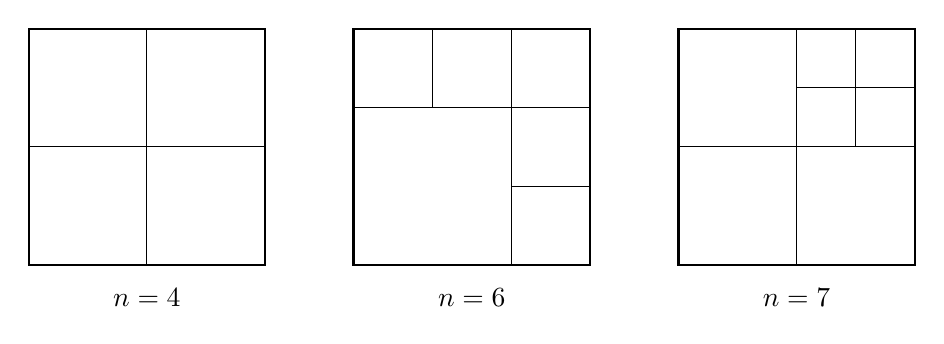
\begin{tikzpicture}[scale=0.75]
% n = 4
\begin{scope}[xshift=0cm]
  \draw[thick] (0,0) rectangle (4,4);
  \draw (2,0) -- (2,4); \draw (0,2) -- (4,2);
  \node at (2,-0.55) {$n = 4$};
\end{scope}
% n = 6
\begin{scope}[xshift=5.5cm]
  \draw[thick] (0,0) rectangle (4,4);
  \draw (0,0) rectangle (2.6667,2.6667);
  \foreach \y in {0,1.3333} { \draw (2.6667,\y) rectangle (4,\y+1.3333); }
  \foreach \x in {0,1.3333,2.6667} { \draw (\x,2.6667) rectangle (\x+1.3333,4); }
  \node at (2,-0.55) {$n = 6$};
\end{scope}
% n = 7
\begin{scope}[xshift=11cm]
  \draw[thick] (0,0) rectangle (4,4);
  \draw (2,0) -- (2,4); \draw (0,2) -- (4,2);
  \draw (3,2) -- (3,4); \draw (2,3) -- (4,3);
  \node at (2,-0.55) {$n = 7$};
\end{scope}
\end{tikzpicture}

\vspace{0.6cm}

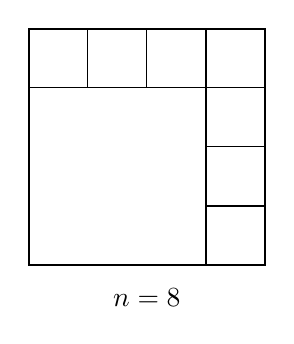
\begin{tikzpicture}[scale=0.75]
% n = 8
\begin{scope}
  \draw[thick] (0,0) rectangle (4,4);
  \draw (0,0) rectangle (3,3);
  \foreach \y in {0,1,2,3} { \draw (3,\y) rectangle (4,\y+1); }
  \foreach \x in {0,1,2} { \draw (\x,3) rectangle (\x+1,4); }
  \node at (2,-0.55) {$n = 8$};
\end{scope}
\end{tikzpicture}
\end{center}

\noindent Explicitly:
\begin{itemize}
\item $n = 1$: the square itself.
\item $n = 4$: the $2 \times 2$ grid.
\item $n = 6$: a square of side $\tfrac{2}{3}$ in one corner, plus an L-shaped border of width $\tfrac{1}{3}$ made of $5$ squares of side $\tfrac{1}{3}$. Check: $1 - \tfrac{4}{9} = \tfrac{5}{9} = 5 \cdot \bigl(\tfrac{1}{3}\bigr)^2$.
\item $n = 7$: the $2 \times 2$ grid with one quarter subdivided into four, giving $3 + 4 = 7$.
\item $n = 8$: a square of side $\tfrac{3}{4}$ in one corner, plus an L-shaped border of width $\tfrac{1}{4}$ made of $7$ squares of side $\tfrac{1}{4}$. Check: $1 - \tfrac{9}{16} = \tfrac{7}{16} = 7 \cdot \bigl(\tfrac{1}{4}\bigr)^2$.
\end{itemize}

\subsection*{Part C: the induction}

\textbf{Claim.} For every $n \in \mathbb{N}$ with $n \geq 1$ and $n \notin \{2,3,5\}$, a square can be dissected into $n$ squares.

\medskip
\noindent\textbf{Splitting lemma (the inductive step).} If a square can be dissected into $n$ squares, it can be dissected into $n + 3$ squares. Take any one of the $n$ constituent squares and divide it into four congruent quarter-squares. The count becomes $n - 1 + 4 = n + 3$, and the result is still a dissection into squares. $\square$

\medskip
\noindent\textbf{Proof by strong induction on $n$.}

\medskip
\noindent\emph{Base cases.} $n = 1, 4, 6, 7, 8$ are all constructed explicitly in Part B.

\medskip
\noindent\emph{Inductive step.} Let $n \geq 9$ and assume the claim holds for all $m$ with $1 \leq m < n$ and $m \notin \{2,3,5\}$. Since $n \geq 9$, we have $n - 3 \geq 6$, so $n - 3 \notin \{2,3,5\}$ and $1 \leq n-3 < n$. By the inductive hypothesis a square can be dissected into $n-3$ squares, and by the splitting lemma it can then be dissected into $n$ squares.

\medskip
By strong induction the claim holds for all $n \geq 1$ with $n \notin \{2,3,5\}$. Combined with Part A, the set of counter-examples is exactly $X = \{2,3,5\}$. $\blacksquare$

\medskip
\noindent Note that the splitting lemma increases the number of squares by exactly $3$, so from a single starting value it reaches only one residue class modulo $3$. The base cases $6$, $7$ and $8$ cover all three residues, which is why three of them are required.

\section*{Question 9}

\textbf{Language.} Alphabet $\{a, b, c, |, \times\}$. Formulas: $a$, $b$, $c$ are formulas; if $\psi$, $\phi$, $\delta$ are formulas then so are $\psi | \phi$ and $\psi \times \phi | | \delta$.

\medskip
\noindent $P(\psi) = $ number of $|$ symbols in $\psi$; \quad $M(\psi) = $ number of $\times$ symbols in $\psi$.

\medskip
\noindent\textbf{Claim.} $\forall \phi.\ P(\phi) \geq 2 M(\phi)$.

\medskip
\noindent\textbf{Proof by structural induction on the formation of $\phi$.}

\medskip
\noindent\emph{Base cases.} $\phi \in \{a, b, c\}$. These contain no $|$ and no $\times$, so $P(\phi) = 0$ and $M(\phi) = 0$. Hence $P(\phi) = 0 \geq 0 = 2M(\phi)$. \checkmark

\medskip
\noindent\emph{Inductive case 1: $\phi = \psi | \chi$.} \\
Inductive hypotheses: $P(\psi) \geq 2M(\psi)$ and $P(\chi) \geq 2M(\chi)$.

Counting symbols, this construction adds exactly one $|$ and no $\times$:
\[
P(\phi) = P(\psi) + P(\chi) + 1, \qquad M(\phi) = M(\psi) + M(\chi).
\]
Therefore
\[
P(\phi) = P(\psi) + P(\chi) + 1 \geq 2M(\psi) + 2M(\chi) + 1 > 2\bigl(M(\psi) + M(\chi)\bigr) = 2M(\phi).
\]
So $P(\phi) \geq 2M(\phi)$. \checkmark

\medskip
\noindent\emph{Inductive case 2: $\phi = \psi \times \chi | | \delta$.} \\
Inductive hypotheses: $P(\psi) \geq 2M(\psi)$, $P(\chi) \geq 2M(\chi)$, $P(\delta) \geq 2M(\delta)$.

This construction adds exactly two $|$ symbols and exactly one $\times$:
\[
P(\phi) = P(\psi) + P(\chi) + P(\delta) + 2, \qquad M(\phi) = M(\psi) + M(\chi) + M(\delta) + 1.
\]
Therefore
\begin{align*}
P(\phi) &= P(\psi) + P(\chi) + P(\delta) + 2 \\
&\geq 2M(\psi) + 2M(\chi) + 2M(\delta) + 2 && \text{by the three inductive hypotheses} \\
&= 2\bigl(M(\psi) + M(\chi) + M(\delta) + 1\bigr) \\
&= 2 M(\phi). \qquad \checkmark
\end{align*}

\medskip
Every formula is built by one of these rules, so by structural induction $P(\phi) \geq 2M(\phi)$ for all formulas $\phi$. $\blacksquare$

\medskip
\noindent The bound is tight, since rule 2 introduces $\times$ and $|$ in the ratio $1 : 2$, so any formula built using only the base cases and rule 2 satisfies $P(\phi) = 2M(\phi)$.

\section*{Question 10}

\begin{enumerate}[label=(\roman*)]

\item \textbf{Natural numbers that are multiples of 7.} Both notations are easy.

\emph{Predicate notation:}
\[
M_7 = \{\, n \in \mathbb{N} \mid \exists k \in \mathbb{N}.\ n = 7k \,\}
\]

\emph{Recursive notation:}
\begin{itemize}
\item $0 \in M_7$;
\item if $n \in M_7$ then $n + 7 \in M_7$;
\item nothing else is in $M_7$.
\end{itemize}

\item \textbf{The prime numbers.} Predicate notation is natural; recursive notation is not.

\emph{Predicate notation:}
\[
\mathrm{Pr} = \{\, n \in \mathbb{N} \mid n > 1 \wedge \forall a, b \in \mathbb{N}.\ (n = ab \iimplies (a = 1 \vee b = 1)) \,\}
\]

\emph{Recursive notation:} there is no easy recursive definition. A recursive definition builds each new element from elements already in the set by a fixed constructor, but a prime is defined by the \emph{absence} of divisors, which is a global negative condition rather than a closure property. The sieve of Eratosthenes is a procedure, not a structural recursion on the set itself. So: no straightforward recursive definition exists.

\item \textbf{Palindromes over $\{0,1\}$.} Both notations are easy.

\emph{Recursive notation:} let $\mathrm{Pal} \subseteq \{0,1\}^*$ be defined by
\begin{itemize}
\item $\varepsilon \in \mathrm{Pal}$, \quad $0 \in \mathrm{Pal}$, \quad $1 \in \mathrm{Pal}$;
\item if $w \in \mathrm{Pal}$ then $0w0 \in \mathrm{Pal}$ and $1w1 \in \mathrm{Pal}$;
\item nothing else is in $\mathrm{Pal}$.
\end{itemize}
(The three base cases are needed because palindromes may have even or odd length.)

\emph{Predicate notation:} writing $w^R$ for the reversal of $w$,
\[
\mathrm{Pal} = \{\, w \in \{0,1\}^* \mid w = w^R \,\}
\]
or, spelling out reversal by indexing, with $|w|$ the length of $w$ and $w_i$ its $i$-th symbol,
\[
\mathrm{Pal} = \{\, w \in \{0,1\}^* \mid \forall i.\ 1 \leq i \leq |w| \iimplies w_i = w_{|w| - i + 1} \,\}.
\]

\item \textbf{The factorial numbers.} Recursive notation is natural; predicate notation is not.

\emph{Recursive notation (as a function):} $f : \mathbb{N} \to \mathbb{N}$ with
\[
f(0) = 1, \qquad f(n+1) = (n+1) \cdot f(n),
\]
and then $F = \{\, f(n) \mid n \in \mathbb{N} \,\}$.

\emph{Recursive notation (as a set, self-contained):} the difficulty is that the next factorial depends on the index as well as the previous value, so carry the index along. Define $S \subseteq \mathbb{N} \times \mathbb{N}$ by
\begin{itemize}
\item $(0, 1) \in S$;
\item if $(n, m) \in S$ then $(n+1, (n+1) \cdot m) \in S$;
\item nothing else is in $S$;
\end{itemize}
then $F = \{\, m \mid \exists n.\ (n,m) \in S \,\}$.

\emph{Predicate notation:} there is no easy predicate definition that avoids reintroducing the factorial function. Writing $F = \{\, m \in \mathbb{N} \mid \exists n \in \mathbb{N}.\ m = n! \,\}$ is circular unless $!$ has already been defined recursively, so predicate notation is not suitable here.

\item \textbf{The square numbers.} Predicate notation is natural; recursive notation is less direct.

\emph{Predicate notation:}
\[
\mathrm{Sq} = \{\, n \in \mathbb{N} \mid \exists k \in \mathbb{N}.\ n = k^2 \,\}
\]

\emph{Recursive notation:} as with the factorials, the step depends on the index, since $(k+1)^2 = k^2 + 2k + 1$. Carrying the index, define $S \subseteq \mathbb{N} \times \mathbb{N}$ by
\begin{itemize}
\item $(0, 0) \in S$;
\item if $(k, n) \in S$ then $(k+1,\ n + 2k + 1) \in S$;
\item nothing else is in $S$;
\end{itemize}
then $\mathrm{Sq} = \{\, n \mid \exists k.\ (k,n) \in S \,\}$. A recursive definition on the set of values alone is not easy, because the increment between consecutive squares is not constant.
\end{enumerate}

\section*{Question 11}

\subsection*{(i)}

\begin{center}
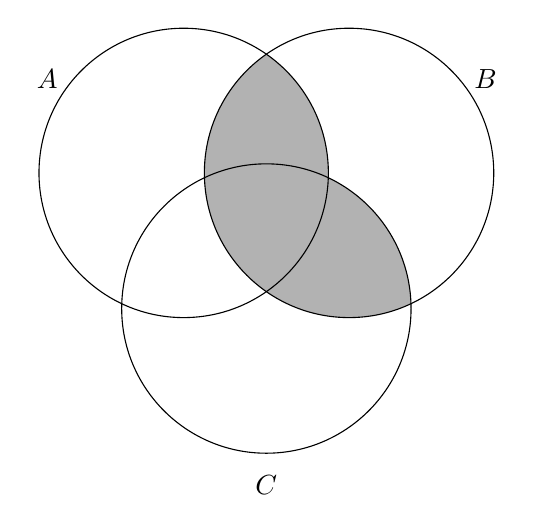
\begin{tikzpicture}[scale=1.05]
  \def\ra{1.75}
  \coordinate (A) at (-1,0.62);
  \coordinate (B) at (1,0.62);
  \coordinate (C) at (0,-1.02);
  % shade A cap B
  \begin{scope}
    \clip (A) circle (\ra);
    \fill[black!30] (B) circle (\ra);
  \end{scope}
  % shade B cap C
  \begin{scope}
    \clip (C) circle (\ra);
    \fill[black!30] (B) circle (\ra);
  \end{scope}
  \draw (A) circle (\ra);
  \draw (B) circle (\ra);
  \draw (C) circle (\ra);
  \node at (-2.65,1.75) {$A$};
  \node at (2.65,1.75) {$B$};
  \node at (0,-3.15) {$C$};
\end{tikzpicture}
\end{center}

\noindent\textbf{Regions shaded:} $A \cap B \cap \overline{C}$ (region 4), $A \cap B \cap C$ (region 7), and $\overline{A} \cap B \cap C$ (region 6). Everything inside $A$ alone, inside $C$ alone, inside $B$ alone, and the lens $A \cap C \cap \overline{B}$ is unshaded.

\medskip
\noindent Taking the union of those three regions and simplifying:
\[
\bigl((A \cap B) \setminus C\bigr) \;\cup\; (A \cap B \cap C) \;\cup\; \bigl((B \cap C) \setminus A\bigr)
\;=\; (A \cap B) \cup (B \cap C)
\]
and factoring $B$ out by the distributive law gives the compact form
\[
\boxed{\,(A \cap B) \cup (B \cap C) \;=\; B \cap (A \cup C)\,}
\]

\noindent In words: the elements of $B$ that also belong to at least one of $A$ and $C$.

\subsection*{(ii)}

\begin{center}
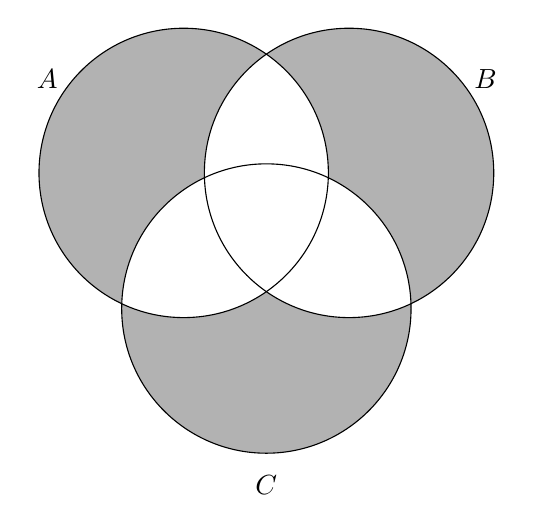
\begin{tikzpicture}[scale=1.05]
  \def\ra{1.75}
  \coordinate (A) at (-1,0.62);
  \coordinate (B) at (1,0.62);
  \coordinate (C) at (0,-1.02);
  % shade all three, then knock out every pairwise overlap
  \fill[black!30] (A) circle (\ra);
  \fill[black!30] (B) circle (\ra);
  \fill[black!30] (C) circle (\ra);
  \begin{scope}
    \clip (A) circle (\ra);
    \fill[white] (B) circle (\ra);
  \end{scope}
  \begin{scope}
    \clip (A) circle (\ra);
    \fill[white] (C) circle (\ra);
  \end{scope}
  \begin{scope}
    \clip (B) circle (\ra);
    \fill[white] (C) circle (\ra);
  \end{scope}
  \draw (A) circle (\ra);
  \draw (B) circle (\ra);
  \draw (C) circle (\ra);
  \node at (-2.65,1.75) {$A$};
  \node at (2.65,1.75) {$B$};
  \node at (0,-3.15) {$C$};
\end{tikzpicture}
\end{center}

\noindent\textbf{Regions shaded:} $A$ only (region 1), $B$ only (region 2), and $C$ only (region 3). Every pairwise overlap and the triple overlap are unshaded, as is the area outside all three circles.

\medskip
\noindent This is the set of elements belonging to \emph{exactly one} of the three sets. Written as a union of the three regions:
\[
\bigl(A \setminus (B \cup C)\bigr) \;\cup\; \bigl(B \setminus (A \cup C)\bigr) \;\cup\; \bigl(C \setminus (A \cup B)\bigr)
\]
Equivalently, take everything in the union and remove everything lying in two or more of the sets:
\[
\boxed{\,(A \cup B \cup C) \setminus \bigl((A \cap B) \cup (A \cap C) \cup (B \cap C)\bigr)\,}
\]

\subsection*{Verification}

The three circles divide the universe into eight disjoint regions, so each expression can be checked region by region. Writing $\checkmark$ for shaded:

\begin{center}
\begin{tabular}{c l c c c c}
\toprule
Region & Description & Diagram (i) & $B \cap (A \cup C)$ & Diagram (ii) & Exactly one \\
\midrule
1 & $A \cap \overline{B} \cap \overline{C}$ & & & $\checkmark$ & $\checkmark$ \\
2 & $\overline{A} \cap B \cap \overline{C}$ & & & $\checkmark$ & $\checkmark$ \\
3 & $\overline{A} \cap \overline{B} \cap C$ & & & $\checkmark$ & $\checkmark$ \\
4 & $A \cap B \cap \overline{C}$ & $\checkmark$ & $\checkmark$ & & \\
5 & $A \cap \overline{B} \cap C$ & & & & \\
6 & $\overline{A} \cap B \cap C$ & $\checkmark$ & $\checkmark$ & & \\
7 & $A \cap B \cap C$ & $\checkmark$ & $\checkmark$ & & \\
8 & $\overline{A} \cap \overline{B} \cap \overline{C}$ & & & & \\
\bottomrule
\end{tabular}
\end{center}

\noindent In both cases the shaded column and the expression column agree in all eight rows, so the two expressions are correct.

\section*{Question 12}

Let $R, S$ be relations on a set $X$ and define
\[
T = \{\, (i,j) \mid \exists k.\ (i,k) \in R \wedge (k,j) \in S \,\}.
\]
This is the composition of $R$ followed by $S$.

\subsection*{(a) If $R$ and $S$ are reflexive, then so is $T$. \quad TRUE}

\noindent\textbf{Proof.} Let $i \in X$ be arbitrary.
\begin{enumerate}
\item Since $R$ is reflexive, $(i,i) \in R$.
\item Since $S$ is reflexive, $(i,i) \in S$.
\item Take the witness $k = i$ in the definition of $T$. Then $(i,k) = (i,i) \in R$ and $(k,j) = (i,i) \in S$ with $j = i$.
\item Hence the existential in the definition of $T$ is satisfied, so $(i,i) \in T$.
\end{enumerate}
Since $i$ was arbitrary, $(i,i) \in T$ for all $i \in X$, so $T$ is reflexive. $\blacksquare$

\subsection*{(b) If $R$ and $S$ are transitive, then so is $T$. \quad FALSE}

\noindent\textbf{Counterexample.} Let $X = \{1,2,3,4,5\}$ and
\[
R = \{(1,2),\ (3,4)\}, \qquad S = \{(2,3),\ (4,5)\}.
\]

\medskip
\noindent\emph{$R$ is transitive.} Transitivity requires: whenever $(x,y) \in R$ and $(y,z) \in R$, also $(x,z) \in R$. The only pairs in $R$ are $(1,2)$ and $(3,4)$. There is no pair in $R$ starting at $2$, and none starting at $4$, so the hypothesis of transitivity is never satisfied. $R$ is vacuously transitive.

\medskip
\noindent\emph{$S$ is transitive.} Same argument: no pair in $S$ starts at $3$ or at $5$, so $S$ is vacuously transitive.

\medskip
\noindent\emph{Computing $T$.}
\begin{itemize}
\item $(1,2) \in R$ and $(2,3) \in S$ give $(1,3) \in T$.
\item $(3,4) \in R$ and $(4,5) \in S$ give $(3,5) \in T$.
\item No other combination matches, so $T = \{(1,3),\ (3,5)\}$.
\end{itemize}

\medskip
\noindent\emph{$T$ is not transitive.} We have $(1,3) \in T$ and $(3,5) \in T$, so transitivity would require $(1,5) \in T$. But $(1,5) \in T$ would need some $k$ with $(1,k) \in R$ and $(k,5) \in S$. The only pair in $R$ starting at $1$ is $(1,2)$, forcing $k = 2$, and $(2,5) \notin S$. Hence $(1,5) \notin T$.

\medskip
Therefore $T$ is not transitive, and the statement is disproved. $\blacksquare$

\end{document}
